\section{Results}

\subsection{IID performance}
\begin{figure}[h]
  \begin{center}
    \includegraphics[width=0.95\textwidth]{./figures/cellot-cohort/iid-predictions.pdf}
  \end{center}
  \caption{caption}
  \label{iid-prediction}
\end{figure}
% TODO: caption
% TODO: text

\begin{figure}[h]
  \begin{center}
    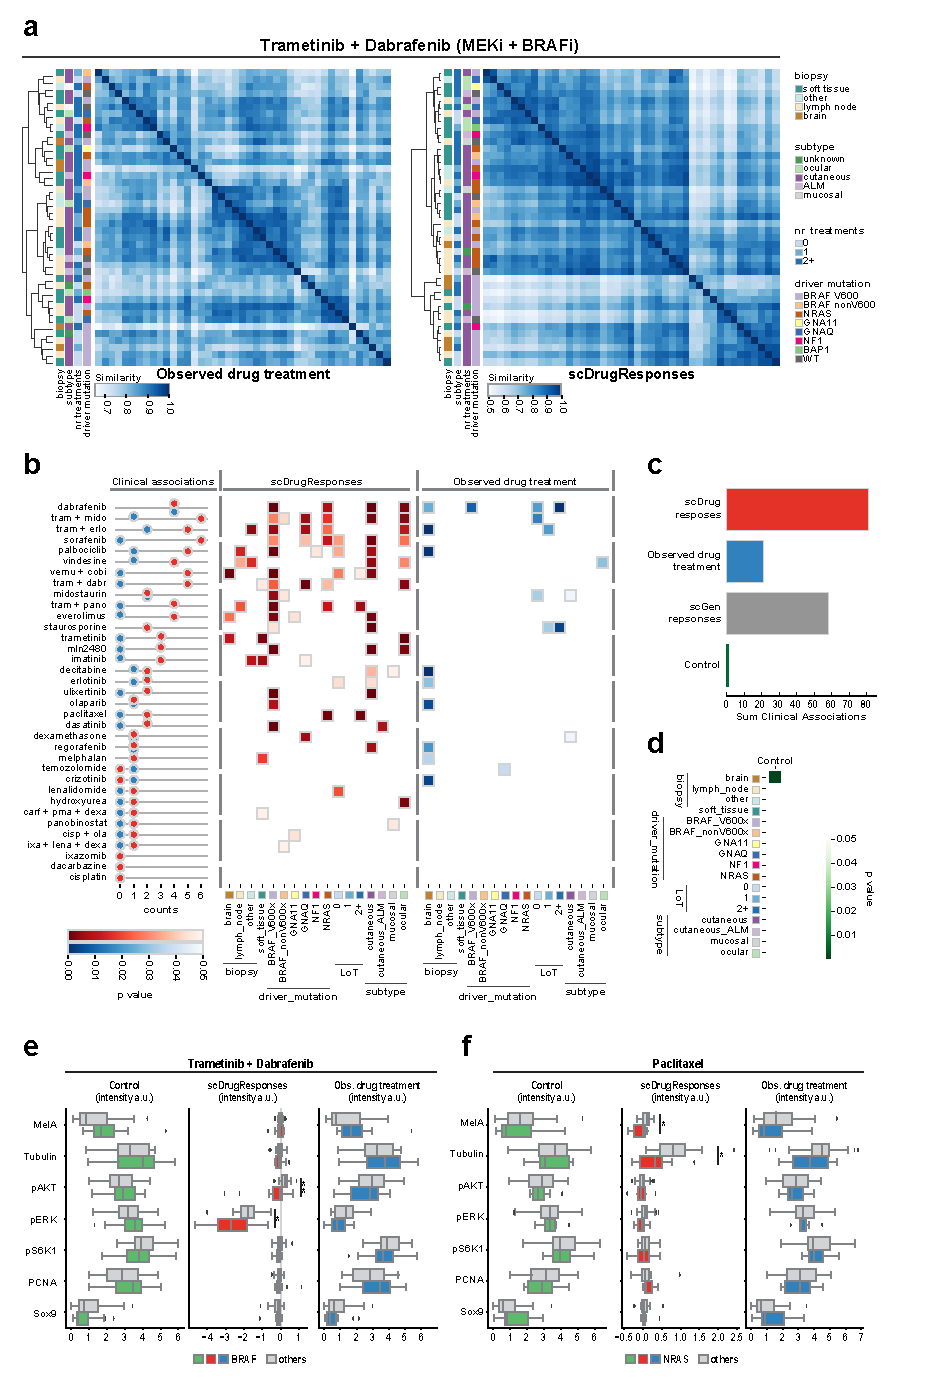
\includegraphics[width=0.95\textwidth]{figures/cellot-cohort/iid-associations.pdf}
  \end{center}
  \caption{caption}
  \label{fig:iid-associations}
\end{figure}
% TODO: caption
% TODO: text

\begin{figure}[h]
  \begin{center}
    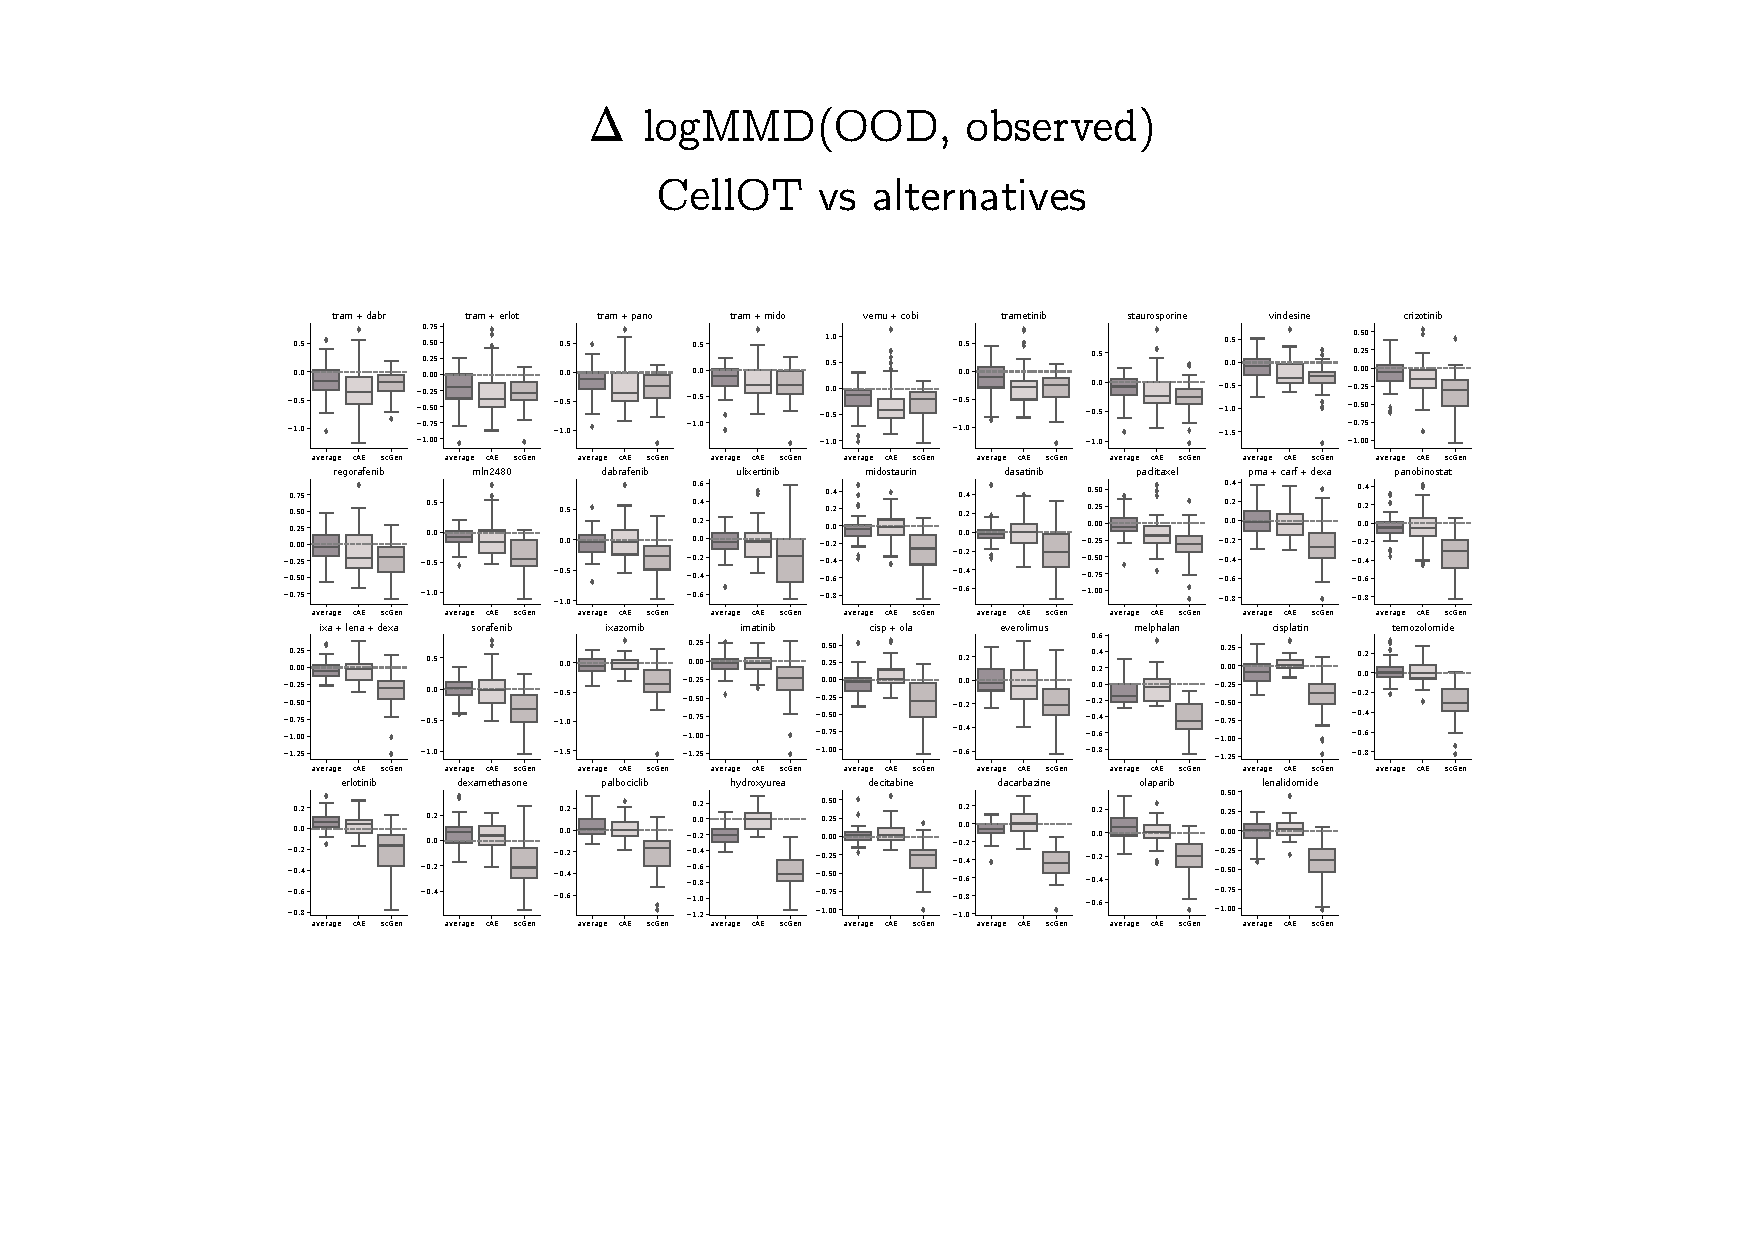
\includegraphics[width=0.95\textwidth]{figures/cellot-cohort/ood-eval-logmmd.pdf}
  \end{center}
  \caption{
    Pairwise logMMD differences comparing $\textsc{CellOT}$ and baseline approaches.
    For each (drug, patient) pair, models are trained on the entire cohort with that patient held out.
    Each model predicts the drug response of the heldout patient
    and logMMD values are computed between the distribution of predicted treated states and the true treated states.
    Negative values correspond to settings where $\textsc{CellOT}$ improves over the corresponding baseline.
  }
\label{fig:ood-eval-logmmd}
\end{figure}

\begin{figure}[h]
  \begin{center}
    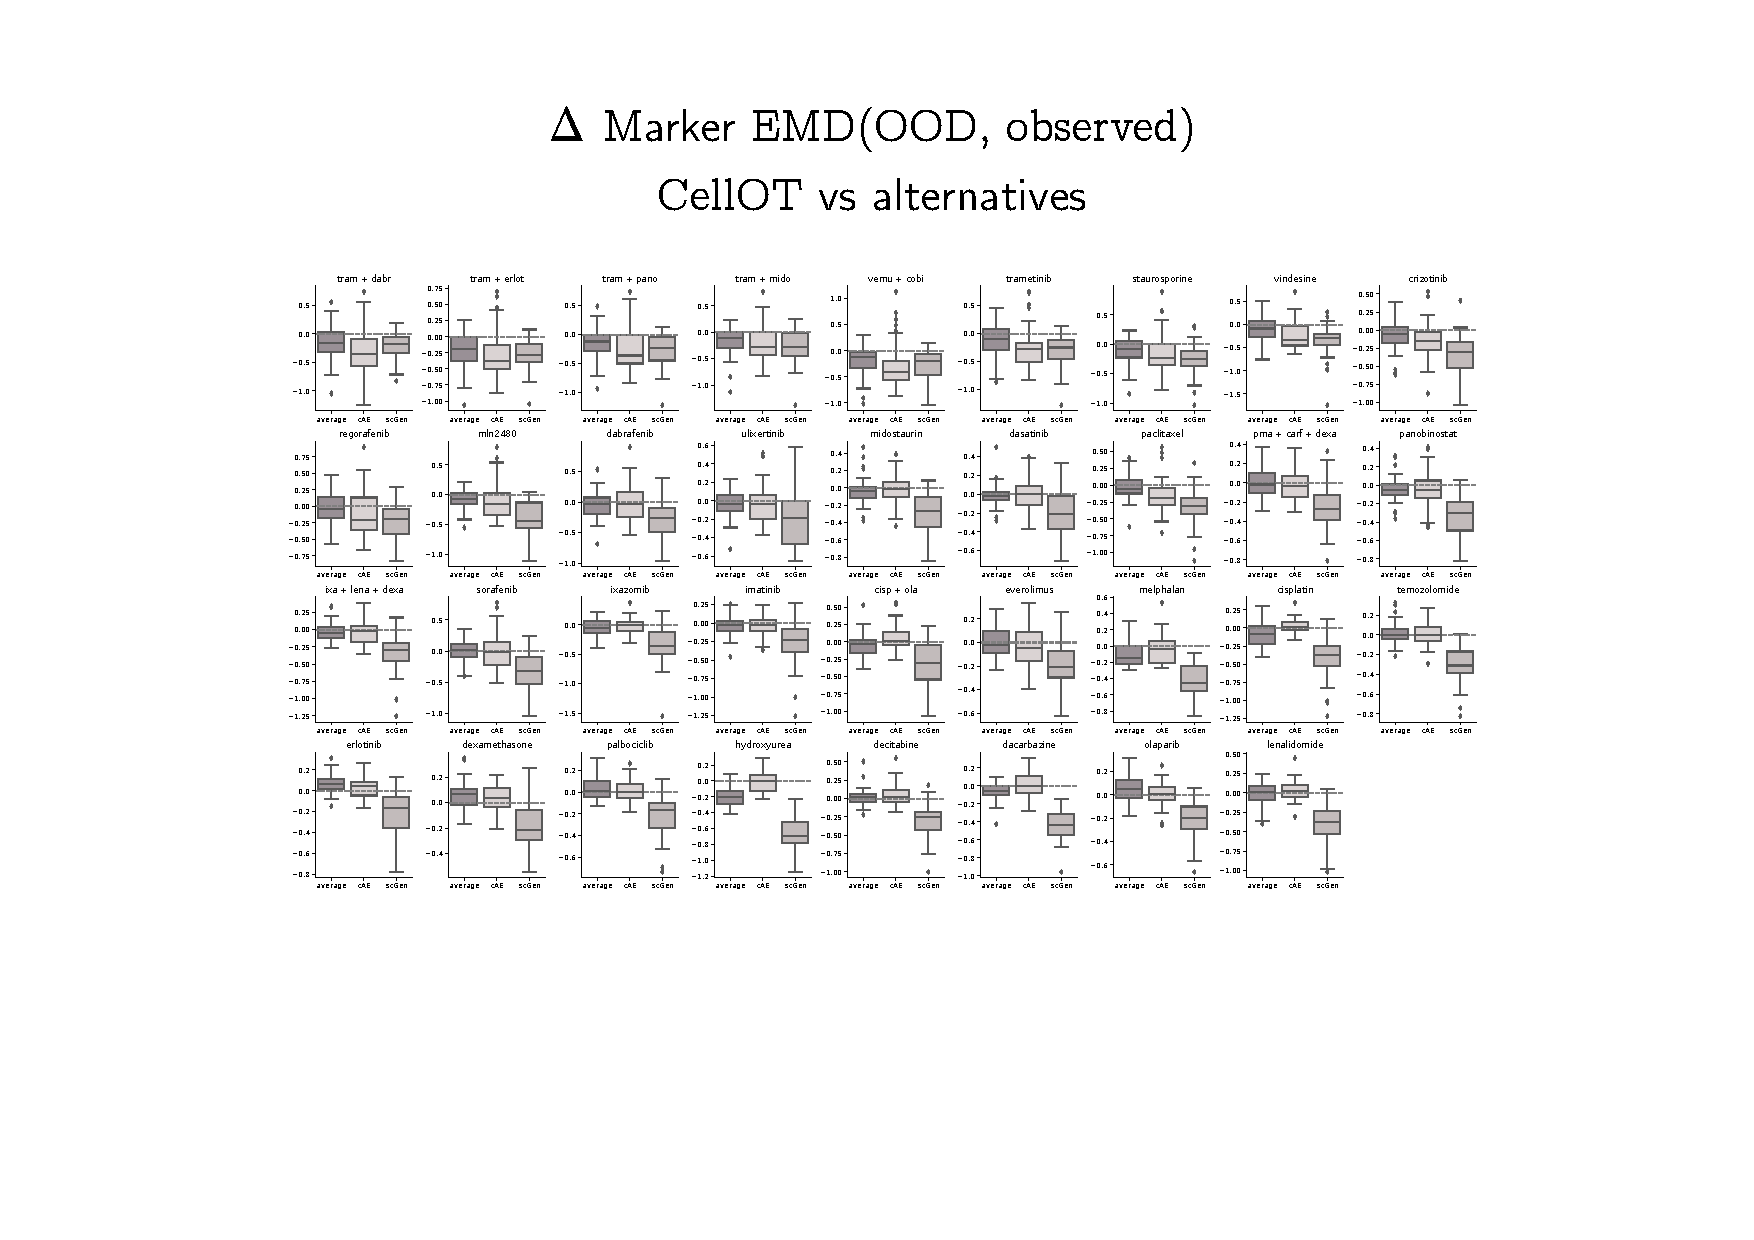
\includegraphics[width=0.95\textwidth]{figures/cellot-cohort/ood-eval-marker.pdf}
  \end{center}
  \caption{
    Pairwise marker EMD differences comparing $\textsc{CellOT}$ and baseline approaches.
    For each (drug, patient) pair, models are trained on the entire cohort with that patient held out.
    Each model predicts the drug response of the heldout patient
    and marker EMD values are computed between the distribution of predicted treated states and the true treated states.
    Negative values correspond to settings where $\textsc{CellOT}$ improves over the corresponding baseline.
  }
  \label{fig:ood-eval-marker}
\end{figure}

\begin{figure}
  \begin{center}
    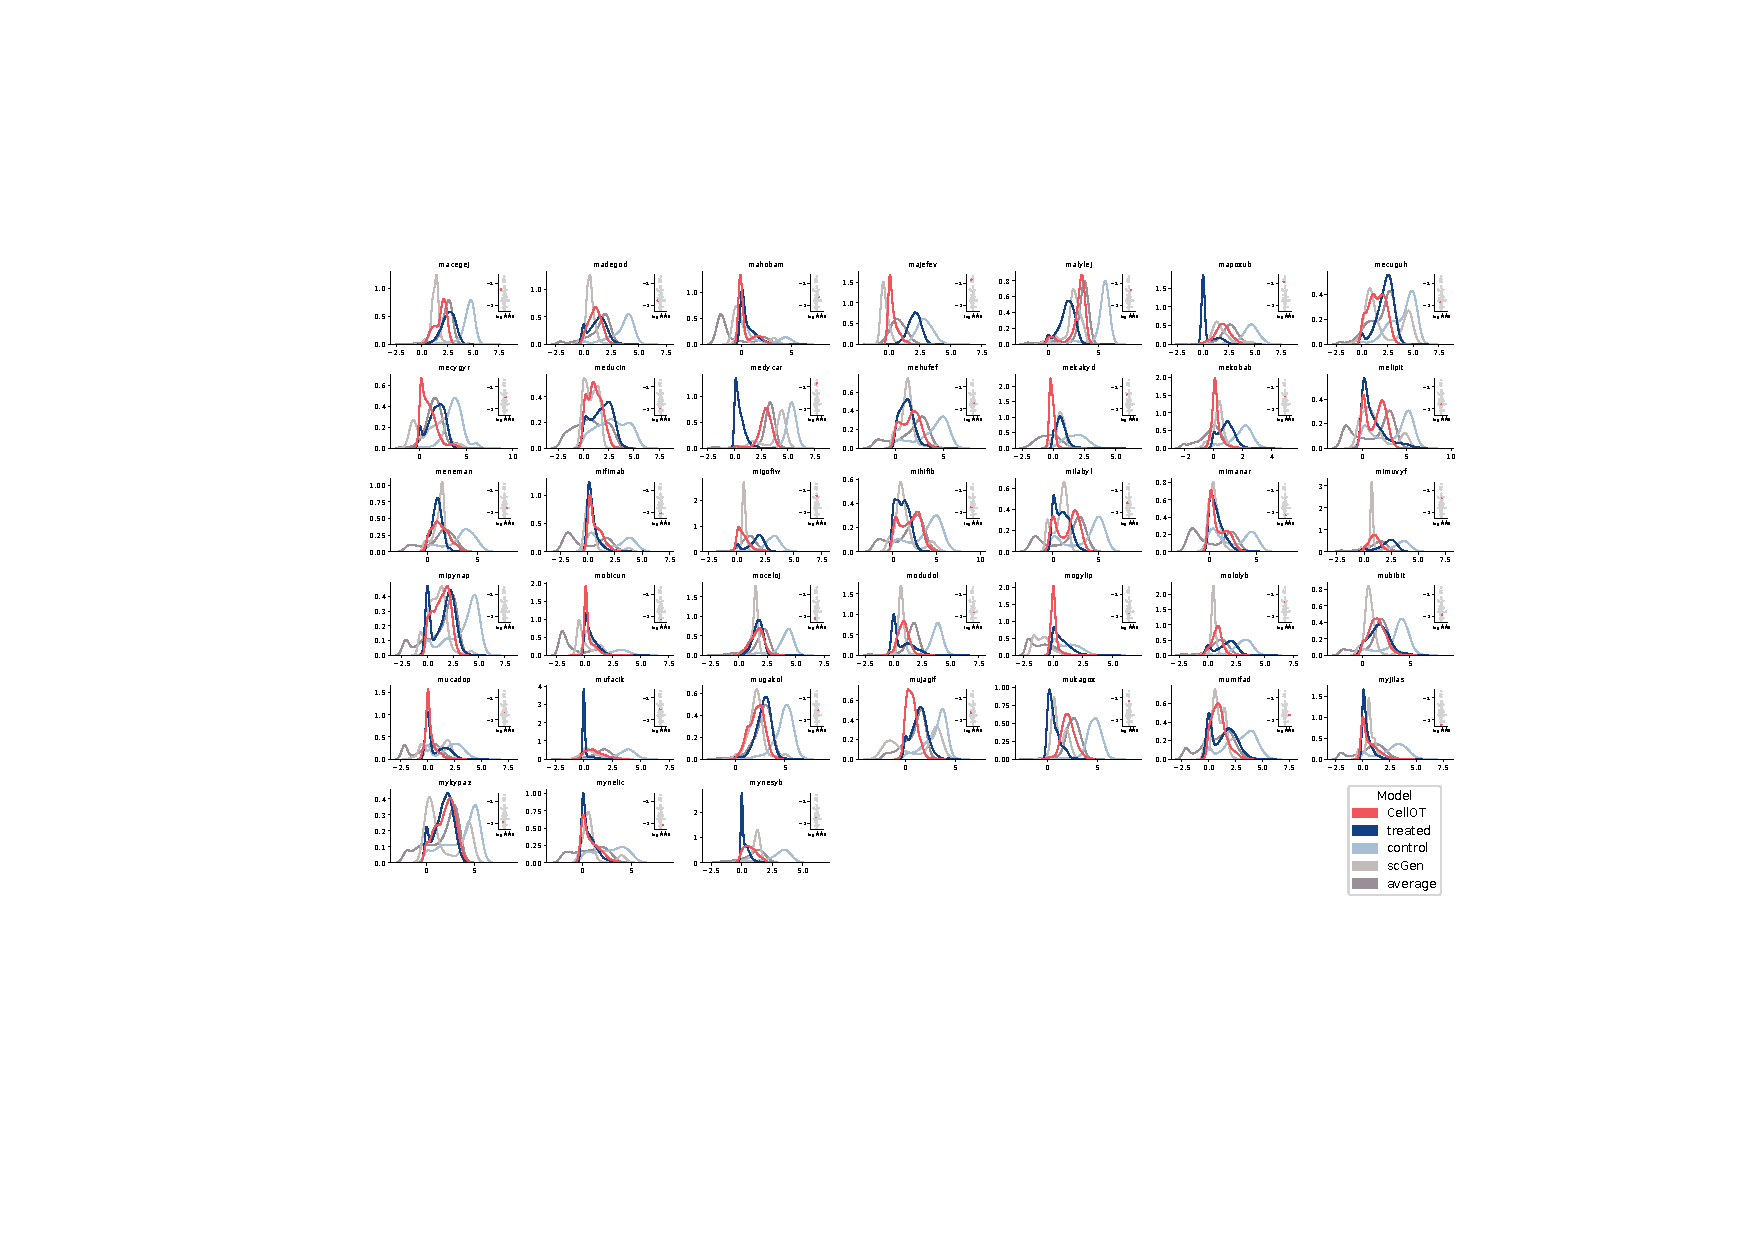
\includegraphics[width=0.95\textwidth]{figures/cellot-cohort/ood-predict-marginals.pdf}
  \end{center}
  \caption{
    Predicted response to trametinib dabrafenib combination treatment of each heldout samples.
    Marginals are shown for the treatment's marker feature, pERK.
    The inlay shows the selected heldout sample's logMMD score against the rest of the cohort.
  }\label{fig:ood-predict-marginals}
\end{figure}

\begin{figure}
  \begin{center}
    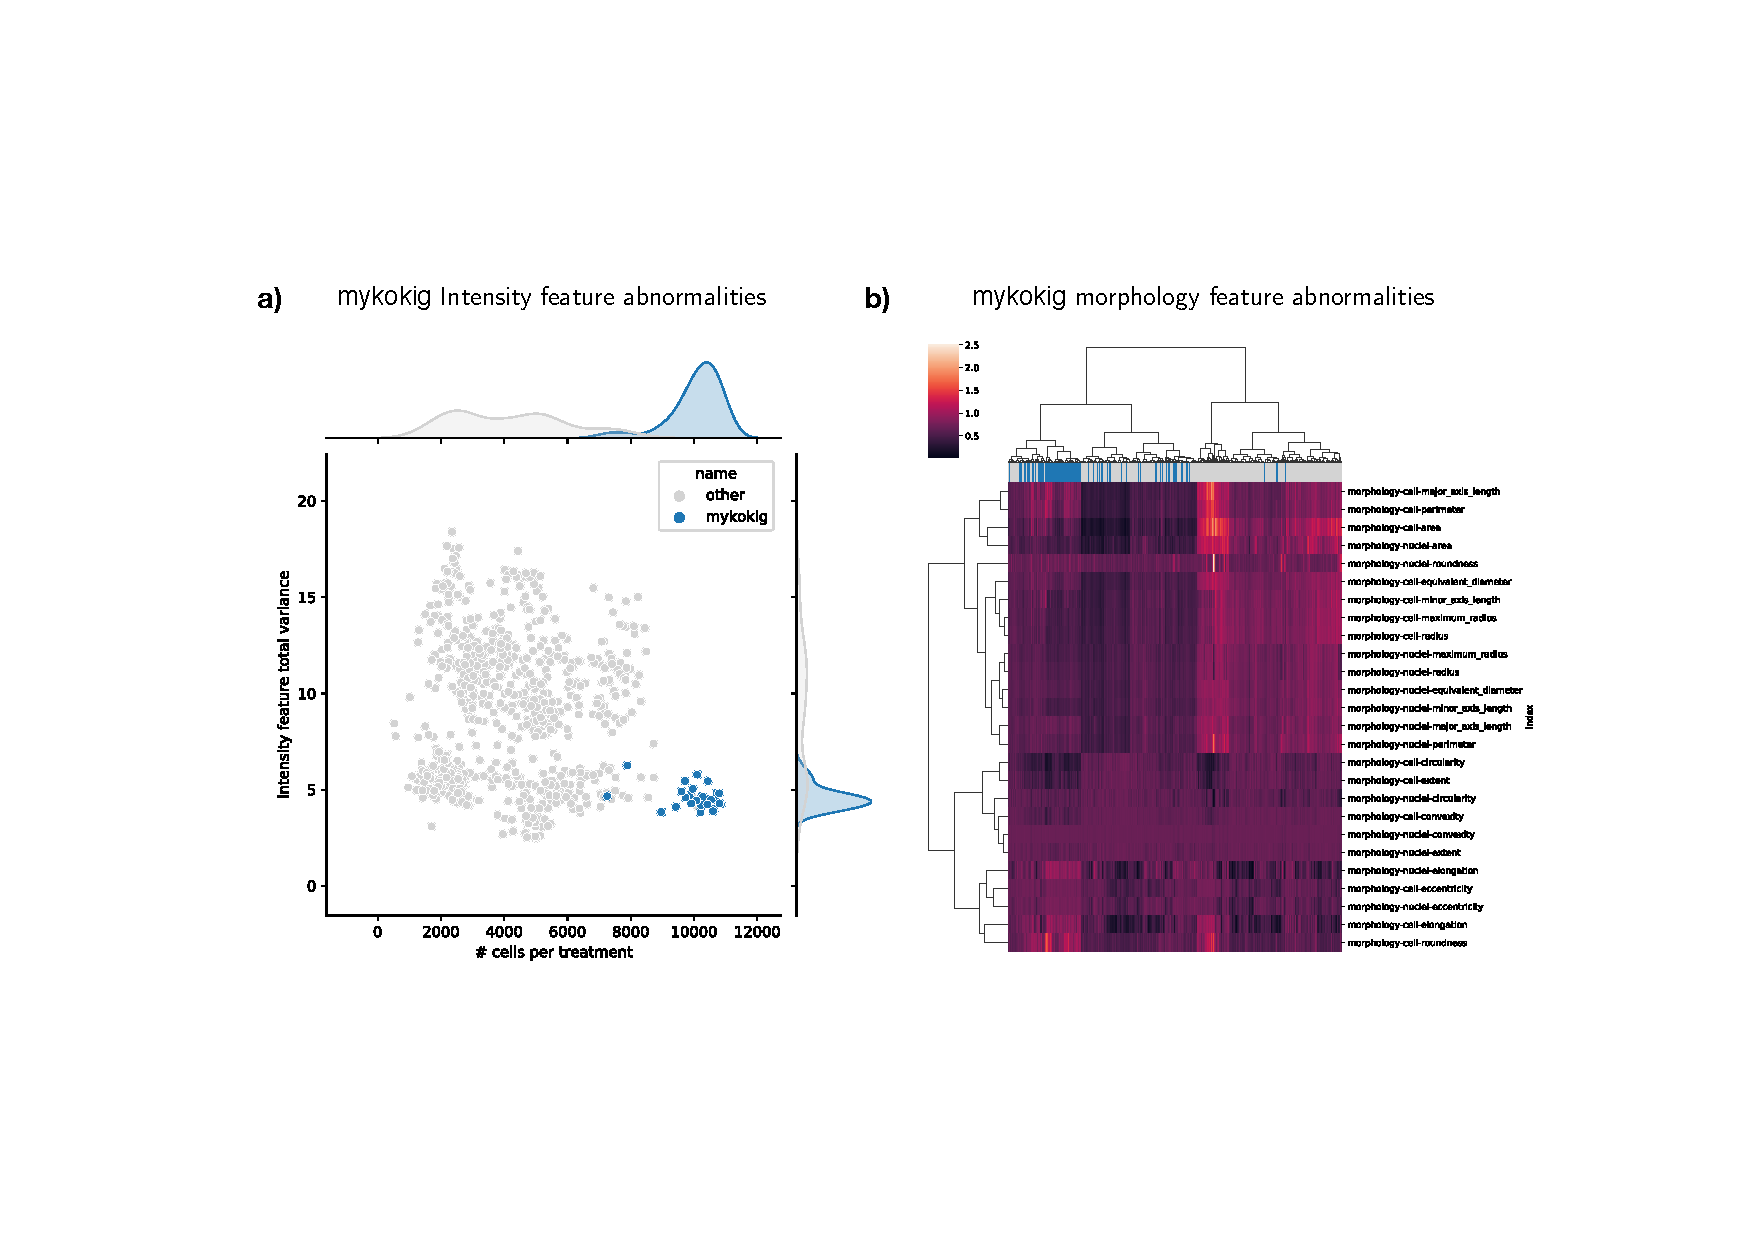
\includegraphics[width=0.95\textwidth]{figures/cellot-cohort/progression-exclude-mykokig.pdf}
  \end{center}
  \caption{
    Sample mykokig exhibits evidence for low quality cell segmentation and is removed from the progression prediction task.
  a) Scatter plot of number of treated cells by the variance of intensity features.  Each dot corresponds to a (treatment, sample) pair and treatments of mykokig are shown in blue. Mykokig behaves as an outlier as it has much more cells per treatment than other samples and these cells have low variance in their intensity features.
  b) Morphology features of mykokig cells indicate the presence of artifacts. The cluster map shows the distribution of each extracted morphology feature (rows) for cells sampled from mykokig and a subset of 5 samples from the full cohort. A large fraction of mykokig cells exhibit a strange unique morphology pattern of small round cells.
  }\label{fig:progression-exclude-mykokig}
\end{figure}

\begin{figure}
  \begin{center}
    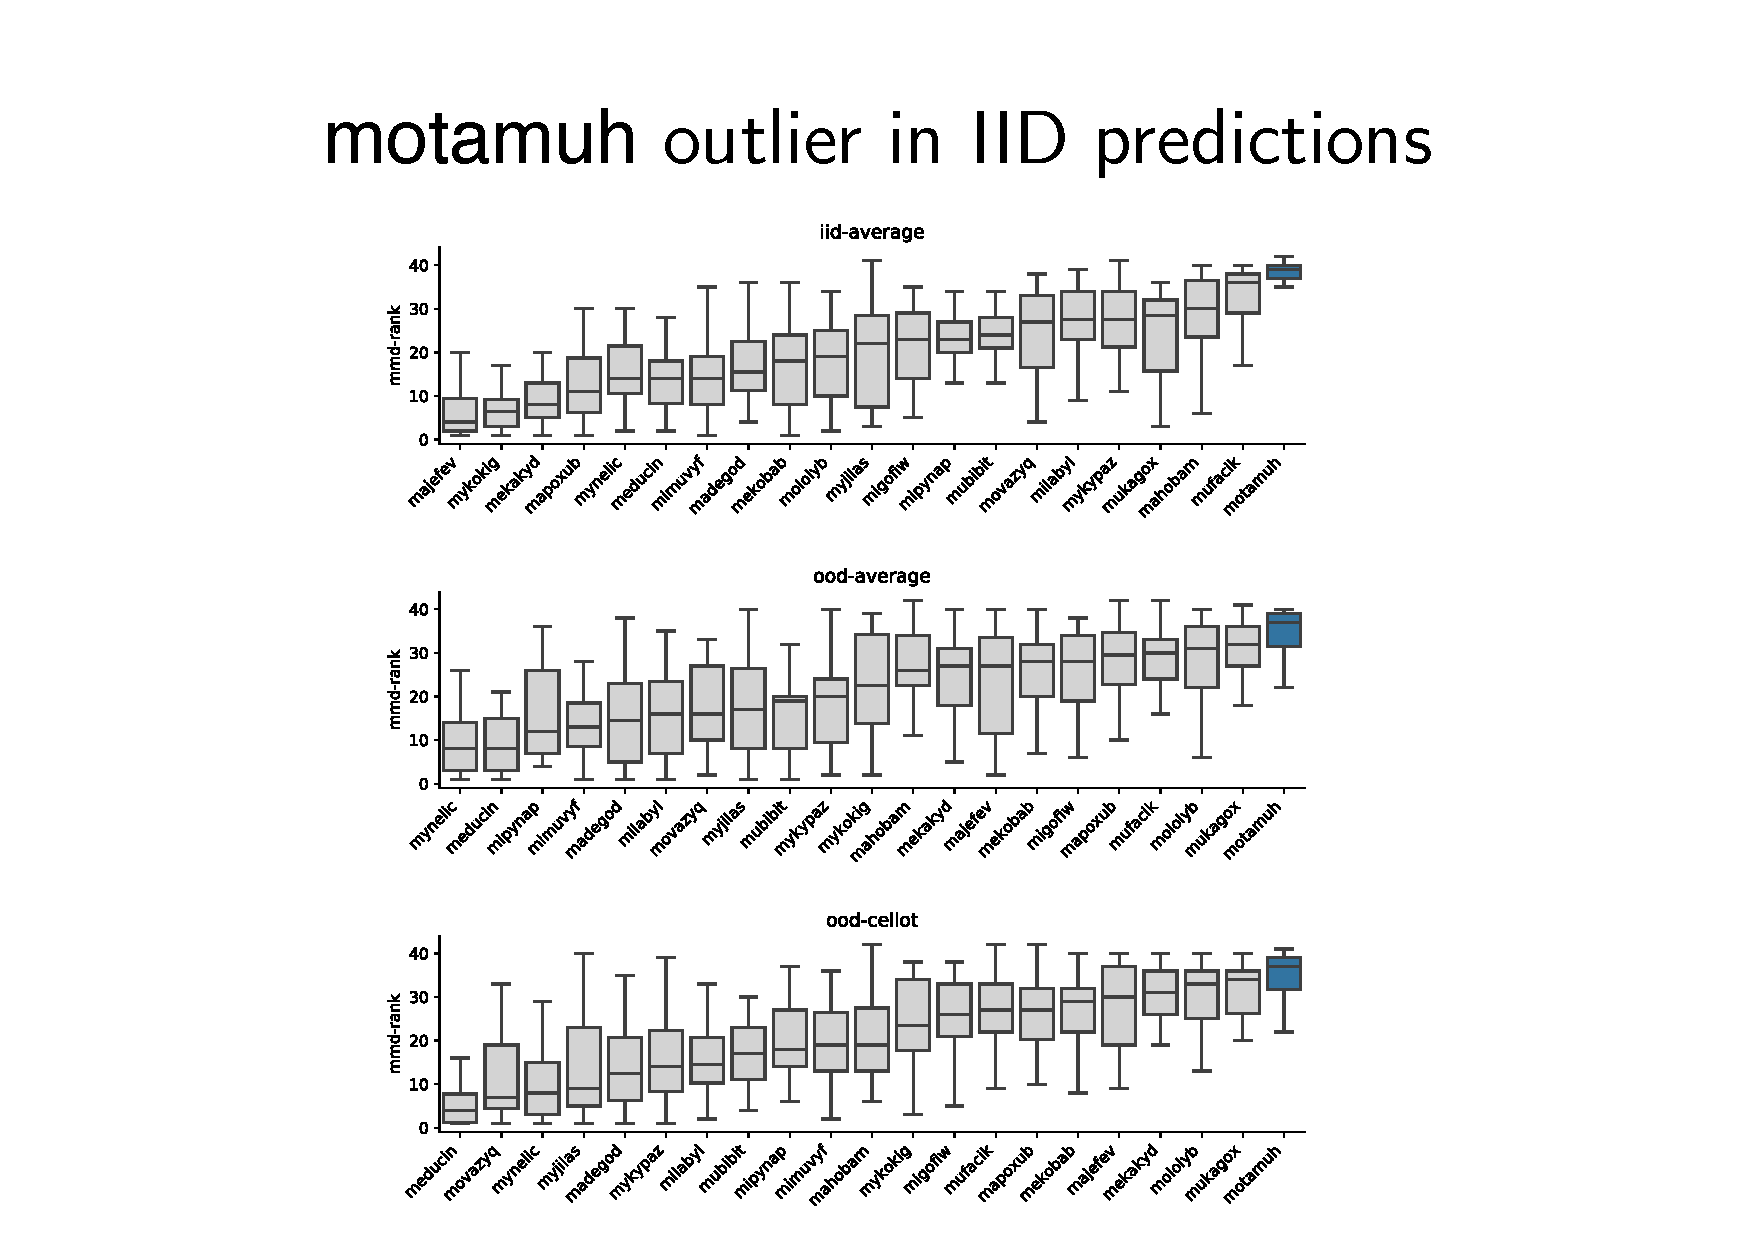
\includegraphics[width=0.95\textwidth]{figures/cellot-cohort/progression-exclude-motamuh.pdf}
  \end{center}
  \caption{
    The predicted responses for sample motamuh are consistently poor and the sample is therefore removed from the progression prediction task.
    Boxplots show the ranked MMD metric computed between each model's prediction and observed treated states for drugs considered in the progression prediction task.
    Results for the average model are shown in the IID and OOD setting as well as CellOT predictions in the OOD setting.
    Sample motamuh consistently ranks worst across all samples in the cohort for these prediction tasks.
  }\label{fig:progression-exclude-motamuh}
\end{figure}

\subsection{OOD performance}
\begin{figure}[ht!]
  \label{fig:ood-main}
  \begin{center}
    \includegraphics[width=0.95\textwidth]{figures/cellot-cohort/ood.pdf}
  \end{center}
  \caption{
    a) Generalization to heldout samples. For each patient, for each drug, we hold that patient out and train a model on the combined set of observed control and treated cells of the rest of the cohort.
    b) Predictions are made on the held out patient for each (patient, drug, model) triplet and metrics are computed between the responses and predictions of the unseen held out patient.
    We report significant differences (t-test, $p < 0.01$) to each baseline model as colored boxes. Blue hues indicate significant improvements.
    The relative treatment strengths, computed as the metric between the observed control and treated cells, are reported as purple column colors.
    c) Selected predicted marginals of marker features.
    The distribution of CellOT-predicted MMD scores is shown in the inlay, highlighting the selected sample.
    d) Predicting the progression status of incoming samples at 90 days using predicted cellular responses.
    Given access to a training subset of the cohort, IID-predicted cellular repsonses are clustered and a binary SVM is trained to classify progression status within 90 days using sample level cluster frequencies.
    Incoming samples are predicted using the \emph{OOD}-predicted cellular responses, i.e. without observations of treated states.
    e) KMeans cluster (k=10) centers of marker intensities cellular responses (left) and the cluster frequencies of each sample (right).
    Column colors correspond to the progression label, misclassification rate, and the known days to progression. Samples close to the cutoff are misclassified.
    f) Accuracy to predict progression status within 90 days of incoming samples.
    We compare against similar approaches which represent cells as their predicted treated state, the observed control state, and a random forest on relevant sample metadata.
  }
\end{figure}

In order to simulate the clinic environment, we construct, for each patient, a training set composed of all other patients in the cohort (Fig \ref{fig:ood-main}a).
Then, for each perturbation available,
we train a model on the control and treated cells across the whole observed cohort
and apply this model to predict the responses of the unseen patient.
We then evaluate the set of predicted cellular states against the unseen treated cells of the held out patient, as we had done in the iid case.
In addition to the MMD metric, which considers the state of a multi-dimensional cellular feature set,
we also report the Earth Mover’s Distance (EMD) of the marker feature of each perturbation.
The marker feature is selected by computing the EMD of the observed control and treated states and selecting the feature with the highest average distance,
i.e. the feature that was most affected by the perturbation.
For instance, for trametinib, this feature is pERK.
The marker feature is of particular interest to the clinician as this typically corresponds to the cellular pathways the treatment is designed to control.

Within each treatment, we compare the ability of CellOT to consistently improve predictions of heldout samples across the whole cohort against baseline approaches.
Fig \ref{fig:ood-main}b shows for which treatments there are significant differences across the whole cohort between
the metric reported by CellOT and the baseline approach, as measured by a relative t-test (p-value < 0.01).
The full distributions for the differences of these metrics can be found in Figures \ref{fig:ood-eval-logmmd} and \ref{fig:ood-eval-marker}.
We demonstrate that we are able to make strong gains in many perturbation settings, including most of the targeted therapies.
These therapies are of particular interest as they are among some of the most commonly administered treatments \cite{need} and, in addition, tend to have the strongest effects.
Many other treatments tend to have more subtle effects, wherein individual effects can dominate the response and thus generalization is difficult to attain.
However, CellOT rarely underperforms against the baselines, and in the few cases when it does, it does so with small effect sizes.
Note that while scGen tends to capture the response of a particular marker feature (EMD metric), it struggles to capture realistic cellular states (MMD metric), while the other baseline methods have the inverse behavior.
CellOT is able to offer the best of both, highlighting its robustness and stability.
We furthermore provide some example marginals (Fig \ref{fig:ood-main}c, full set in Fig \ref{fig:ood-predict-marginals}), showcasing how CellOT is able to learn biologically relevant states.
We include the MMD metric corresponding to the selected CellOT predictions, to give a general indication of how well the model is performing.

\subsection{Learning differential responses with conditional parameters}

\begin{figure}[h]
  \begin{center}
    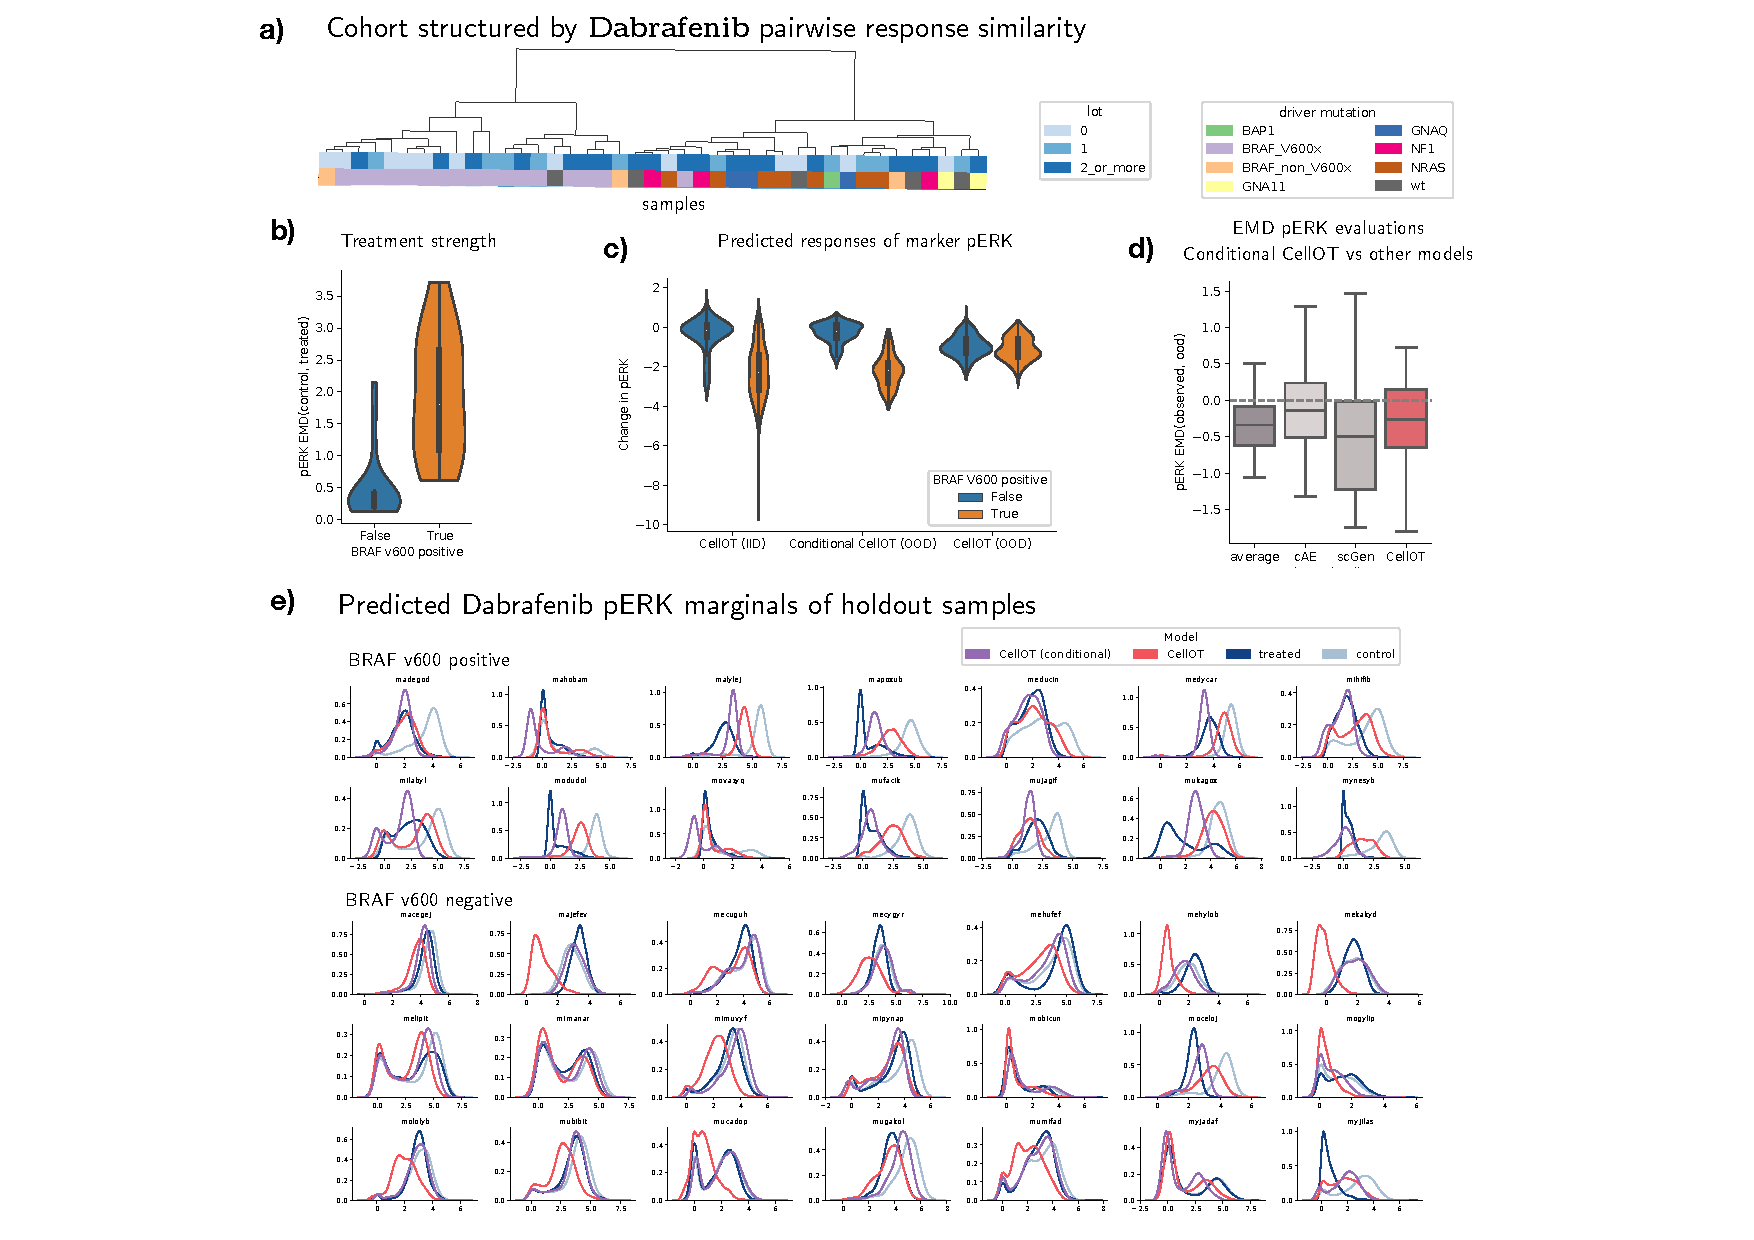
\includegraphics[width=\textwidth]{figures/cellot-cohort/condot.pdf}
  \end{center}
  \caption{
    Predicting strongly differential responses to Dabrafenib of holdout samples using Conditional CellOT.
    a) Dendrogram of sample-level pairwise similarities of Dabrafenib responses, computed using the MMD distances between each sample's distribution of IID-predicted responses reveal similarly responding clusters of non-BRAF samples, BRAF samples with no lines of treatment, and BRAF samples with at least one line of treatment.
    Samples (columns) are colored based on the number of lines of treatment and driver mutation status.
    b) Differential effect strength of Dabrafenib, measured using the EMD of its marker, pERK, between control and treated cells of samples with and without the BRAF driver mutation that the treatment targets.
    c) Predicted responses of pERK for samples with and without the BRAF driver mutation, in both IID and OOD settings.
    OOD $\textsc{CellOT}$ is not able to generalize the differential responses out-of-distribution, while the conditional model has improved performance when compared to the IID model.
    d) Improvements of the pERK marker EMD for predictions made by the conditional CellOT vs other approaches. The metric is computed on the predictions of each approach on cells from holdout samples and the pairwise differences to conditional CellOT are shown. Negative values correspond to improvements Conditional CellOT makes. 
    e) pERK marker marginals for CellOT and conditional CellOT models for BRAF positive (top) and negative (bottom) samples.
  }\label{fig:conditional-ot}
\end{figure}

A common strategy in the design of cancer therapies is to tailor the treatment to interact with some specific mechanism that fails across a number of different cancers.
These \emph{targetted} therapies would, for instance, be designed to treat patients with some driver mutation, such as the infamous BRAF driver mutation \cite{need}.
In such cases, the cellular profile might not capture information crucial to determining the nature of the response, e.g. the presense of the BRAF mutation,
and therefore $\textsc{CellOT}$ performance, as we have described thus far, may struggle.
Here we apply the framework described by \cite{need} to include sample metadata, in the form of \emph{conditional} parameters, in order to help the transport function learn such differential responses.

Here, we focus on the dabrafenib treatment, a targetted therapy to treat BRAF-positive patients.
We observe a strongly differential structure in the responses across the cohort.
Sample similarities are determined by computing the MMD between the learned (IID) single-cell responses of each pair of samples.
Fig \ref{fig:conditional-ot}a) shows a dendrogram computed over the set of these pairwise similarities where were we find three main clusters: non-BRAF samples, BRAF positive samples with no previous lines of treatment, and BRAF positive samples with at least one line of treatment.
While the differential response across BRAF status can be easily explained by the targetted nature of the treatment, the differential resposne to number of treatment lines might be due to a particularly advanced or difficult cancer that necessitates several rounds of treatment.
Fig \ref{fig:conditional-ot}b shows the differential response of pERK, the marker feature for dabrafenib, across BRAF mutation status, by computing the EMD of pERK between the control and observed dabrafenib responses.
Here we observe that dabrafenib induces a strong pERK response in patients with the BRAF mutation, but a weak response in those without,
an observation is in agreement with the intended design and use of the drug.

In order to learn the strongly differential response of dabrafenib,
we train a version of CellOT whose inputs inputs are \emph{conditioned} \cite{condot} with the status of the sample's driver mutation and lines of treatment. 
These conditional parameters are able to inform and influence its learned responses with clinical metadata
This is acheived by concatenating a one-hot encoding of each metadata to the cellular features.
Note that while the potentials trained by $\textsc{CellOT}$ must be convex in their inputs,
they do not need to be convex in these conditional inputs \cite{icnn}.

By comparing the conditional $\textsc{CellOT}$ predictions to vanilla $\textsc{CellOT}$ trained in the IID and OOD settings, we observe that the conditional version is able to better capture the differential pERK responses.
In Fig \ref{fig:conditional-ot}c) we see that the IID $\textsc{CellOT}$, which is able to learn patient-specific responses, indicates that BRAF samples respond to dabrafenib by decreasing pERK levels, while non-BRAF samples have a negligible response.
OOD $\textsc{CellOT}$, on the other hand, predicts all samples, regardless of their BRAF status, to respond to dabrafenib with a slight decrease of pERK levels, and report little to no difference across BRAF status.
The conditional $\textsc{CellOT}$, however, is able to correctly predict a differential response across BRAF status.
This is futher quantified in Fig \ref{fig:conditional-ot}d), where we see consistent improvement in OOD pERK prediction when using conditional $\textsc{CellOT}$ over vanilla $\textsc{CellOT}$ and other baseline models.
Finally, marginals highlighting the learned differential responses are shown in Fig \ref{fig:conditional-ot}e,
where it can been seen that conditional $\textsc{CellOT}$ indeed learns the pERK response of BRAF positive samples (top) and non-response of negative (bottom).

\subsection{Identifying at-risk patients from predicted cellular responses}
The ability to understand whether or not a tumor will progress quickly is of clinical importance as it is an indicator of the severity of the cancer.
In this experiment we demonstrate the clinical utility of predicted single-cell perturbation responses of incoming patients by classifying the progression status of this sample 90 days after treatment.
Here, we simulate the clinic enviornment, and assume that we have access to the control and perturbed states from a (training) cohort.
Given an incoming sample, we observe only their untreated cells, \emph{predict} their cellular responses using the OOD $\textsc{CellOT}$ maps described above, and finally identify the progression status from a model trained on the observed responses of the cohort.

\paragraph{Subcohort selection}
To ensure that we select treatments that are relevant to the situation of individual patients, we limit ourselves to the treatments that had been prescribed to samples by the medical board associated with the Tumor Profiler project.
From the total cohort, 22 samples had been prescribed a studied small molecule treatment.
Of these 22, we removed three samples due to quality control: \textsc{mykokig}, had evidence of unfiltered artifacts in its observed treated cells \ref{fig:progression-exclude-mykokig}, \textsc{motamuh}, as it represents an extreme outlier in IID and OOD response prediction tasks \ref{fig:progression-exclude-motamuh} , and \textsc{mecygyr}, as it had showed evidence of immediate progression at the start of the study ( $<$ 5 days), leaving a subcohort of 19 samples.
Of these 19, 9 progress within 90 days and 10 do not, which yields a balanced binary prediction task.
We simulate the clinic environment by splitting the patients into a train (75\%) and test (25\%) set, (i.e. within each split, 4 of the 19 samples are heldout), where we have access to the control and treated cells of all patients in the training set, and can only access the control cells of patients in the testset.

\paragraph{Prediction model}
Our prediction model, summarized in Fig \ref{fig:ood-main}d, works as follows: first, single-cell responses are clustered and patients are represented as frequencies over these clusters, and then an SVM classification model is trained to predict the binary progression status using the patient representations.
To construct the patient representations of the training set, a KMeans clustering is computed using the single-cell treatment responses from all patients in the training set, as predicted using the IID CellOT models \ref{}.
We perform a soft assignment of each cell to the k cluster centers, via a softmax transformation over the negative distances to each cluster center, to smooth cluster assignments and help include a notion of cluster similarities, Fig \ref{fig:ood-main}e left.
After this step, each cell is now represented as a probability over the set of cluster centers, Fig \ref{fig:ood-main}e right.
A patient-level representation is constructed by averaging the cluster assignments over all cells from each patient.
At test time, the OOD-predicted cell responses are used instead of the IID, as we are unable to access their treated cell states.
The predicted responses are mapped to the cluster centers, the sample frequencies are computed and the held out sample is classified with the SVM.
Note that the visualizations in Fig \ref{fig:ood-main}e are constructed on IID responses of all samples in the subcohort.
Within each split, these structures are re-computed on the training set only.

\paragraph{Evaluation}
Since this is a balanced classification task, we report accuracy as our metric and consider 50\% a trivial lower bound.
For each model setting we perform 100 75\%-25\% train-test splits, i.e. in each split, 4 of the 19 samples are heldout.
We include a model that predicts the progression stats at 90 days with meta information at the sample level, specifically a random forest over the subtype, lines of treatment, and known driver mutation, represented as the concatenation over one-hot encodings of each category.
We furthermore compare our approach to a similar approach that uses predicted treated states, control cells, and single-cell responses predicted by the baselines \ref{}.

The prediction accuracy of holdout samples over 100 train-test splits are shown in Fig \ref{fig:ood-main}f, where we compare using single-cell responses to using control and (predicted) treated states.
In addition, we include a random forest model trained on relevant metadata information, the sample’s subtype, known driver mutation and lines of treatment.
% TODO: fill with actual numbers
The random forest trained on sample metadata and SVM classification using control states only struggle to peform, yielding accuracies of XXX +/- XX.
The SVM classification using treated states fares slightly better, reporting accuracies of XXX +/- XX.
We see the most drastic improvement using \emph{response} information, which reports accuracies of XXX +/- XX.
% TODO: add fig
Comparisons to the autoencoder approaches as well as ablations over the number of clusters can be found in Fig \ref{}, where we show specifically that $\textsc{CellOT}$ responses are stable with respect to classification parameters and out perform baseline approaches.

A benefit of using a straight-forward clustering approach is the ability to interpret the behavior of the model.
We can interpret the decisions made by the model by analyzing the cluster means and patient frequencies over them shown in Fig \ref{fig:ood-main}e.
Here, progression status at 90 days and the misclassification rate of test set samples are shown as row colors.
We see that cells from cluster 5 exhibit a general non-response to the selected perturbations.
Furthermore, samples that have high representation of these responses are more likely to progress,
while samples that exhibit higher degrees of heterogeneity in response are shown to have a better progression status.

